\usecaseristoratore{Modifica informazioni ristorante}
\label{usecase:Modifica informazioni ristorante}

\begin{figure}[h]
	\centering
	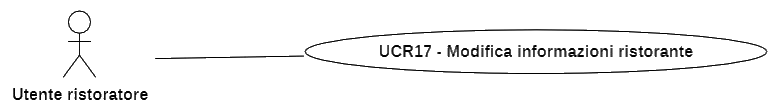
\includegraphics[width=0.9\textwidth]{./uml/UCR17.png} 
	\caption{Modifica informazioni ristorante}
	\label{fig:UCR17}
  \end{figure}

\begin{itemize}
	\item \textbf{Attore principale:} Utente ristoratore.

	\item \textbf{Precondizione:} L'Utente ristoratore ha effettuato l'accesso al Sistema (vedi \autoref{usecase:Effettua accesso}).

	\item \textbf{Postcondizione:} L'Utente ristoratore modifica le informazioni del proprio ristorante.


	\item \textbf{Scenario principale:}
	      \begin{enumerate}

		      \item Il Sistema mostra le informazioni del ristorante:
		      \begin{itemize}
                \item Nome ristorante.
                \item Orario del ristorante.
                \item Descrizione del ristorante.
                \item Indirizzo del ristorante.
                \item Recapiti del ristorante.
                \item \textit{Password}. 
                \item \textit{Link} al sito del ristorante.
                \item Nome ristoratore.
                \item Costo ristorante.
                \item Disponibilità di sedie per bambini (numero).
                \item Adatto a persone con ridotta mobilità.
              \end{itemize}

		      \item L'Utente ristoratore può modificare le informazioni del suo ristorante;
		      \item Il Sistema registra le modifiche apporate alle informazioni dal ristoratore.

	      \end{enumerate}
\end{itemize}
